\section{Експериментальна кампанія на типовій CI}
\label{sec:exp}

\subsection{Постановка та дизайн}

Кампанія виконується у публічному continuous-integration робочому процесі на
чотириядерному хост-раннері з 16~ГБ. Обмежена CI --- заплановане середовище
калібрування: доступне, відтворюване й придатне, коли виділені кластери
недоступні. Кожне завдання розгортає мережу Hyperledger Besu~\cite{besu} QBFT із
$\n$ валідаторами за протоколом \RNM{} (Означення~\ref{def:rnm}). Замкнений
генератор задає~$\cc$ конкурентних відправників і фіксує усталену committed
пропускну здатність після прогріву. Відмови ін'єктуються через kernel traffic
control (omission і duplication; не equivocation).

\textbf{X1}/\textbf{X3} калібрують $(\beta,\gamma)$ на факторній сітці;
\textbf{X2} перевіряє режим квот; \textbf{X3b} повторно семплює вздовж шляхів
конкурентності; \textbf{X4} змінює емульований RTT; \textbf{X5} звітує частоти
детектора; \textbf{X7}/\textbf{X8} перевіряють покриття прогнозних інтервалів і
абляцію визначення розміру. Крос-клієнтна реплікація (\textbf{X9}/GoQuorum) поза
межами. Разом $\resTotalRuns$ успішних записів,
$\approx\resCoreHours$ core-годин, $\n_{\max}=\resNmaxMeasured$.

\paragraph{Відтворюваність.}
Усі експерименти відтворювані з публічного CI-робочого процесу та архівованих
артефактів за адресою
\url{https://github.com/bpenyak/Resource_Normalized_Scaling_Laws_for_Byzantine_Consensus}.

\subsection{Результати}

\emph{X1/X3 --- двофакторне калібрування.}
Спільний МНК на $\resCalibNobs$ ненасичених прогонах без відмов при опорній
квоті ($\n\in\{4,\dots,16\}$, $\cc\in\{1,\dots,16\}$) дає
$\beta=\resBeta\pm\resBetaSE$ і $\gamma=\resGamma\pm\resGammaSE$
($R^{2}=\resRsq$; табл.~\ref{tab:results}) за фіксованої конкурентності та
$\q=0.25$; підгонка використовує всі~$\n$, включно з відкладеними. Сталий
$\beta$ --- усереднення: локальні нахили при $\cc=16$ дорівнюють
$\approx\resBetaLocalA$, $\resBetaLocalB$, $\resBetaLocalC$ на $\n=4$--$7$,
$7$--$13$, $13$--$16$, а переоцінки на $\n\le\resSmallNmax$ дають
$\beta=\resBetaCalibMaxN$ (об'єднані квоти) і $\resBetaSmallN$ (опорна квота),
на $\resBetaGapCalib$ і $\resBetaGapSmallN$ стандартної похибки менше.
Посилення спаду пояснюємо залишковою конкуренцією на хості, коли резервація
$\n\q$ наближається до чотирьох ядер, спільних із генератором навантаження:
\RNM{} усуває конкуренцію лише доки $\n\q$ менше за кількість ядер хоста.
Основне $\beta$ консервативне щодо $\nmax$, але оптимістичне щодо
$\kappaScale$: вікно $[4,4]$ за побудовою однакове для обох підгонок, а
переоцінка на $\n\le\resSmallNmax$ підвищує $\kappaScale$ з $\resKappa$ до
$\resKappaSmallN$.

\emph{X3b --- перевірка шляху Пропозиції~\ref{prop:identifiability}.}
Однофакторна підгонка вздовж $\lambda=1$ дає $\ahat=\resAlphaHat$ проти
$\gamma\lambda-\beta=\resAlphaPred$.
Рис.~\ref{fig:confounding} показує, що виміряні показники відстежують
$\gamma\lambda-\beta$ --- узгодженість з аналітичним передбаченням, а не
універсальна істинність двофакторної форми. Передбачена зміна знака
($\lambda\approx\resLambda$) лежить поза перевіреними $\lambda\in\{0,1,2\}$,
тож перевірка стосується величини зсуву, а не самої зміни знака.

\begin{figure}[!t]
\centering
\begin{minipage}[t]{0.32\textwidth}
\centering
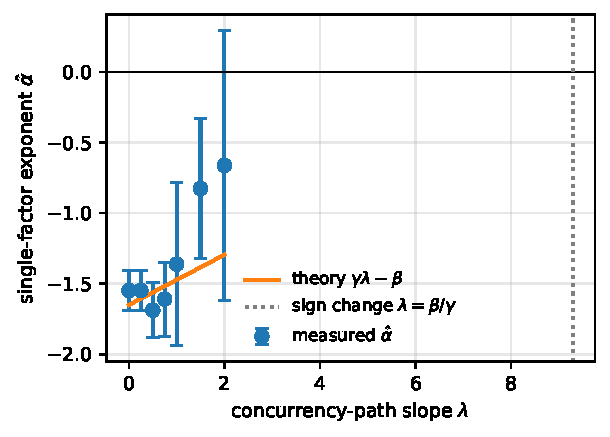
\includegraphics[width=\textwidth]{figures/fig_confounding}
\caption{Виміряні $\ahat$ (точки) проти аналітичного $\gamma\lambda-\beta$
(лінія) (Пропозиція~\ref{prop:identifiability}); передбачена зміна знака при
$\lambda=\resLambda$, поза перевіреними шляхами}
\label{fig:confounding}
\end{minipage}\hfill
\begin{minipage}[t]{0.31\textwidth}
\centering
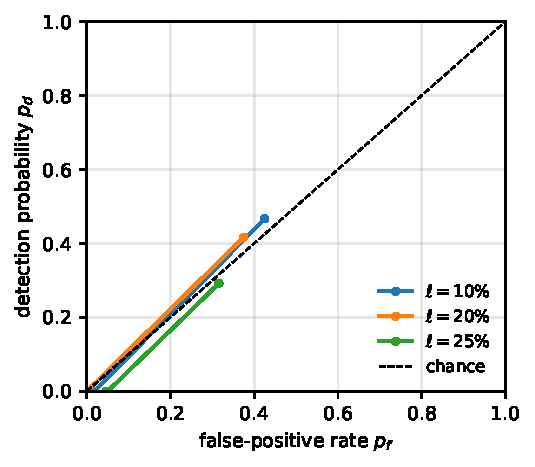
\includegraphics[width=\textwidth]{figures/fig_roc}
\caption{Виміряна ROC детектора (AUC$\,=\,\resAuc$, майже випадковий рівень);
детекційне обмеження з ним невиконуване}
\label{fig:roc}
\end{minipage}\hfill
\begin{minipage}[t]{0.32\textwidth}
\centering
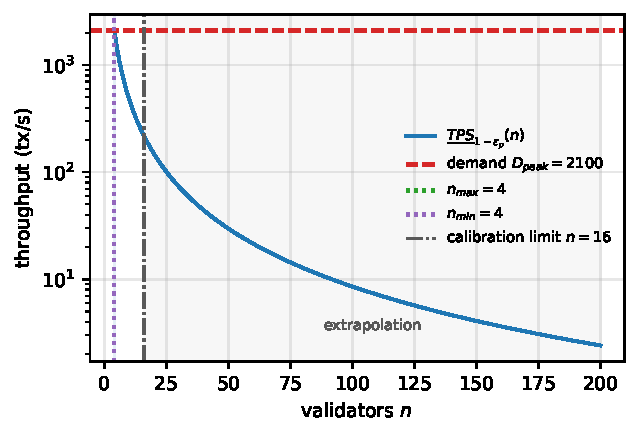
\includegraphics[width=\textwidth]{figures/fig_window}
\caption{Сценарій~A: нижня межа PI пропускної здатності vs.\ $\n$ при
$\kappaScale=\resKappa$; вікно $[\resNminCase,\resNmaxCase]$; штрихпунктир:
межа калібрування $\n=\resNmaxMeasured$}
\label{fig:window}
\end{minipage}
\end{figure}

\emph{X2 --- режим квот.}
X2 вимірює $\n\in\{4,7,13\}$ при $\cc=16$. Частковий $F$-тест взаємодії
квота\,$\times\log\n$ відхиляє спільний нахил ($p=\resQinvP$): $\beta$
дорівнює $\resBetaQlow$ і $\resBetaQmid$ при $\q=0.20,0.25$, але
$\resBetaQhigh$ при $\q=0.33$. У комірках $\q=0.33$ пропускна здатність при
$\n=4$ вже не зростає з квотою ($\resTpsQlowNfour$, $\resTpsQmidNfour$,
$\resTpsQhighNfour$~TPS), що вказує на не-CPU стелю, яка порушує
Припущення~\ref{as:separable}, а при $\n=13$ резервація $\approx4.3$ ядра
перевищує ємність хоста, тобто виходить за Означення~\ref{def:rnm}. Отже,
\RNM{} стабілізує $\beta$ за фіксованої квоти в CPU-обмеженому режимі, але не
робить його незалежним від квоти; коефіцієнти звітовано при $\q=0.25$.

\emph{X4 --- затримка.}
На власній сітці ($\n\in\{7,13\}$, $\cc=16$, $\q=0.25$) X4 дає
$\beta=\resBetaRttZero$ при $0$~мс і $\resBetaRttHigh$ при $200$~мс RTT
($\Delta\beta=\resDeltaBetaRtt$). Базове значення --- двоточковий нахил за
чотирма прогонами; воно узгоджується зі спільною підгонкою $\beta=\resBeta$ у
межах $1.3$ стандартної похибки. Проміжні RTT немонотонні
(табл.~\ref{tab:results}), тож X4 показує напрям і приблизну величину
WAN-штрафу, а не закон залежності від затримки.

\emph{X5 --- детектор.}
За $\resDetRuns$ прогонами з ін'єкцією відмов об'єднана ROC має
AUC$\,=\,\resAuc$ (рис.~\ref{fig:roc}, майже випадковий рівень); $\rho$ з цих
прогонів не ідентифікується і покладається рівним~$0$. За цих частот
детекційне обмеження невиконуване і його послаблено (не застосовується)
(підрозділ~\ref{sec:detection}).

\begin{table}[!t]
\centering
\caption{Калібровані параметри, перевірка квот, детектор і покриття
(досліджене розгортання)}
\label{tab:results}
\scriptsize
\begin{tabular}{lll}
\headline
Величина & Оцінка & Примітка \\
\headline
$\Tzero$; $\beta$; $\gamma$ &
  $\resTzero$; $\resBeta\pm\resBetaSE$; $\resGamma\pm\resGammaSE$ &
  двофакторна \\
$\csat$, $\theta$; $\hat\sigma$ & $\resCsat$, $\resTheta$; $\resSigmaRes$ &
  насичення / залишок \\
$\ahat$ при $\lambda=0,1,2$ &
  $\resAlphaHatLzero$, $\resAlphaHatLone$, $\resAlphaHatLtwo$ &
  X3b \\
$\beta$ при $q=0.20,0.25,0.33$ &
  $\resBetaQlow$, $\resBetaQmid$, $\resBetaQhigh$ &
  X2, $p=\resQinvP$ \\
$\beta$ при RTT $0,25,50,100,200$~мс &
  $\resBetaRttZero$, $\resBetaRttTwentyFive$, $\resBetaRttFifty$,
  $\resBetaRttHundred$, $\resBetaRttHigh$ &
  X4, $\n\in\{7,13\}$ \\
$\hat p_{d}$, $\hat p_{f}$ (частоти позначення); $J$; AUC &
  $\resPd$, $\resPf$; $\resYouden$; $\resAuc$ &
  X5, поріг $\resDetectorThr$ \\
покриття $90\%$/$95\%$ &
  $\resCovHitsNinety/\resHoldoutRuns$, $\resCovHitsNinetyFive/\resHoldoutRuns$ &
  підгонка $\n\le\resCalibMaxN$; hold-out $\resHoldoutN$ \\
\headline
\end{tabular}
\end{table}

\emph{X7/X8 --- покриття, порівняння та абляція.}
Окрема переоцінка на $\resCalibRuns$ прогонах без відмов з
$\n\le\resCalibMaxN$, яка не бачить відкладених прогонів, дає інтервали, що
покривають $\resCovHitsNinety$ і $\resCovHitsNinetyFive$ з $\resHoldoutRuns$
прогонів ($\resHoldoutN$) на рівнях $90\%$ і $95\%$. Перевірка груба
(більшість прогонів при $\n=13$, квоти X2 об'єднано, біноміальна похибка
$\approx6$~п.п.; $\n=11$ не має вигляду $3f+1$) і стосується процедури
інтервалів, а не основного $\beta=\resBeta$.
Позавибіркова log-RMSE для лінійного / однофакторного / USL~\cite{gunther2007} /
двофакторного прогнозів становить $\resRmseLinear$, $\resRmseSingle$,
$\resRmseUsl$, $\resRmseOurs$; однофакторний прогноз тут трохи точніший лише
тому, що всі відкладені прогони мають $\cc=16$. Відносні вартості визначення
розміру: $\resCostLinear$, $\resCostSingle$, $\resCostUsl$, $\resCostOurs$.
